\chapter{Introdução}\label{introducao}
% determinacao da potencia sonora

Várias técnicas de controle de ruído e vibrações foram desenvolvidas nesses últimos tempos visando oferecer um ambiente agradável, principalmente no que diz respeito a dissipassão de energia de vibração em elementos estruturais. Para tanto há 2 análises possíveis a se fazer do elemento estrutural: funções resposta em frequência (FRF's) e coeficientes de amortecimento. 

Em vista do que foi exposto, esse trabalho tem como objetivo determinar e analisar o comportamento das funções resposta em frequência (FRF's) e coeficientes de amortecimento. Para determinação e análise das funções resposta em frequência serão objetos de estudo uma viga engastada e uma placa suspensa, uma excitada por uma martelada e outra por um $shaker$ transmissor de ruído branco respectivamente. Para a determinação e análise dos coeficientes de amortecimento, será objeto de estudo uma placa fina que será submetida, dado os parâmetros corretos de entrada, aos cálculos de decaimento de energia e a banda de meia potência.

\chapter{Fundamentação Teórica}\label{fundamentacao}

Segundo \cite{lenzi2009modelos} funções resposta em frequência (FRF) são tipos de funções transferência que associa um sinal de entrada num sistema (por exemplo força) a um sinal de saída que pode ser a aceleração, velocidade ou deslocamento de um ponto de interesse de uma estrutura. Existem diversos tipos de FRF's que podem ser divididas em grupos dependendo do tipo de grandeza associada:
\begin{itemize}
	\item Receptância ou rigidez dinâmica: deslocamento/força ou força/deslocamento respectivamente;
	\item Mobilidade ou impedância mecânica: velocidade/força ou força/velocidade respectivamente;
	\item Inertância ou massa aparente: aceleração/força ou força/aceleração respectivamente.
\end{itemize}

Experimentalmente as FRFs podem ser adquiridas utilizando-se de transdutores piezelétricos de aceleração (acelerômetros) e de força (martelo/cabeça de impedância/célula de carga) específicos para o contexto de vibrações. Os transdutores convertem o sinal da grandeza física medida (direta ou indiretamente) em um sinal de tensão elétrica proporcional a grandeza mensurada. Os sinais fornecidos pelos transdutores são enviados a um amplificador, convertidos para o domínio digital-discreto e depois a um software de pós-processamento dos dados no intuito de obter as informações de interesse. Vale ressaltar que normalmente o processamento de dados tem como base a transformada de fourier visto que a maioria dos fenômenos de vibrações são mais visíveis no domínio da frequência. Para esse contexto foi medido a inertância da viga engastada e da placa suspensa, uma função resposta em frequência (FRF) obtida a partir da razão da transformada de fourier (FFT) da aceleração ao longo do tempo pela transformada de fourier (FFT) da força ao longo do tempo.

No que diz respeito ao método do decaimento é necessário definir qual equação que rege a vibração de um sistema massa-mola-amortecedor. Normalmente sistemas massa-mola-amortecedor com movimentos repetitivos (vibratórios) são regidos pela equação

\begin{equation}  
	x(t) = X_{o}e^{-\xi\omega_{n}t}e^{j\omega_{d}t},
\end{equation}
tal que $X_{o}$ é a amplitude máxima do movimento vibratório, $\xi$ é a razão de amortecimento (quanto maior $\xi$, menor será o tempo do elemento estrutural entrar em estado estacionário), $\omega_{n}$ é a frequência natural do sistema e $\omega_{d}$ frequência natural amortecida (frequência no qual o amortecimento irá atuar). Para a definição da frequência natural do sistema usa-se a fórmula 
\begin{equation}
	\omega_{n} = \sqrt{\frac{k}{m}},
\end{equation}
tal que $k$ é o coeficiente de rigidez do sistema e $m$ é a massa. Para o cálculo da frequencia de amortecimento pode-se fazer do uso da fórmula 
\begin{equation}
	\omega_{d} = \omega_{n}\sqrt{1 - \xi}.	
\end{equation}

Vale ressaltar também que a energia vibratória é proporcional ao módulo do deslocamento de tal forma que $E(t) \propto e^{-2\xi\omega_{n}t}$. E, considerando que o tempo de reverberação $T_{60}$ da estrutura é o tempo em que relatada energia decai em 60 dB, o coeficiente de amortecimento $\eta$ de um elemento estrutural massa-mola-amortecedor é dada pela equação 
\begin{equation}
	\eta = \frac{3}{\pi f_{n}T_{60}log_{10}e},
\end{equation}
tal que $e$ é uma constante cujo valor aproximado é $e \cong 2,7181$ e $f_{n}$ a frequência natural do enésimo modo.

\chapter{Experimento e Equipamentos}\label{descricao}

Para realizar as medições utilizou-se os seguintes instrumentos:

\begin{itemize}
	\item dois microfones;
	\item um calibrador de microfone;
	\item dois rotating boom;
	\item um computador
	\item um analisador de sinais modelo SCADAS da LMS;
	\item uma placa de teste (1800 mm x 1130 mm x 2 mm);
	\item uma fonte sonora;
	\item um amplificador de potência;
	\item uma fonte Sonora de referência.
\end{itemize}

E o esquemático das câmaras I e II, geradora e receptora respectivamente, foi constituída de acorda com a figura \ref{experimento_1}.

\begin{figure}[h]
	\centering
	%\hspace{-4.5cm}
	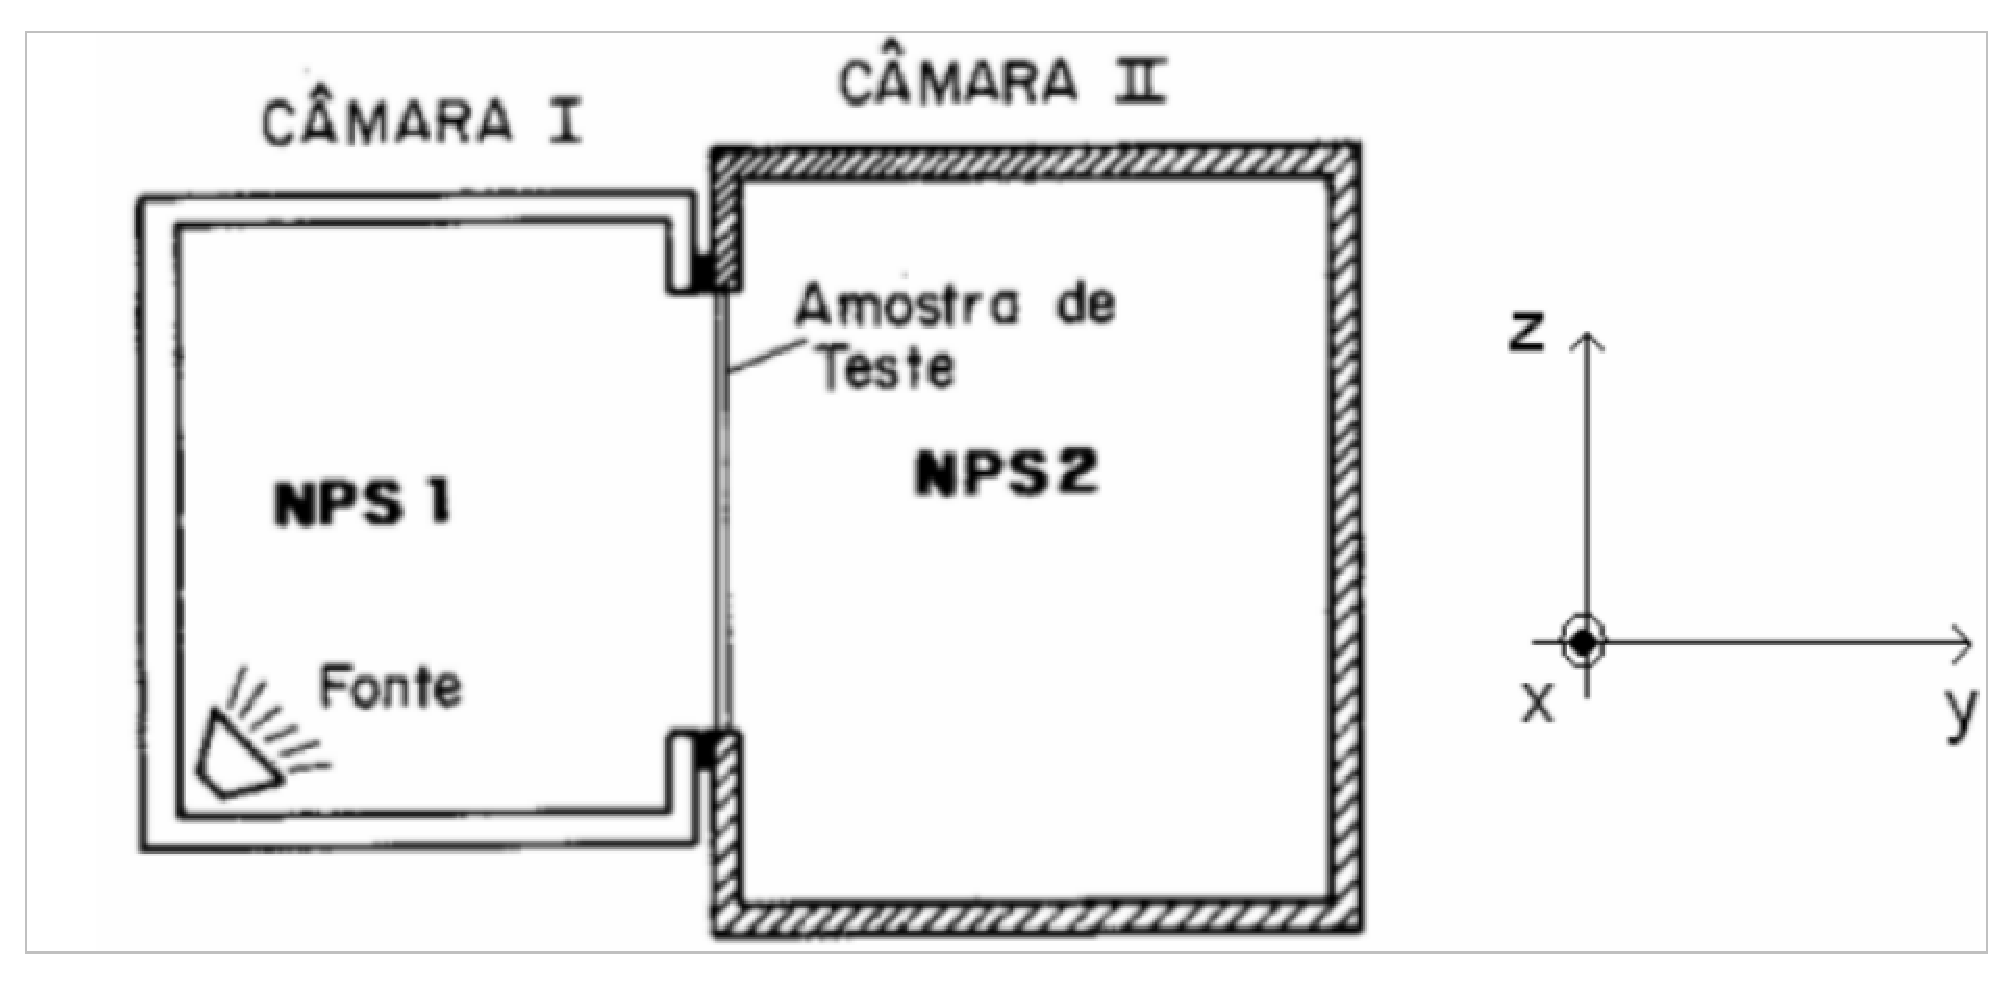
\includegraphics[scale=0.28]{imagem_3.eps}
	%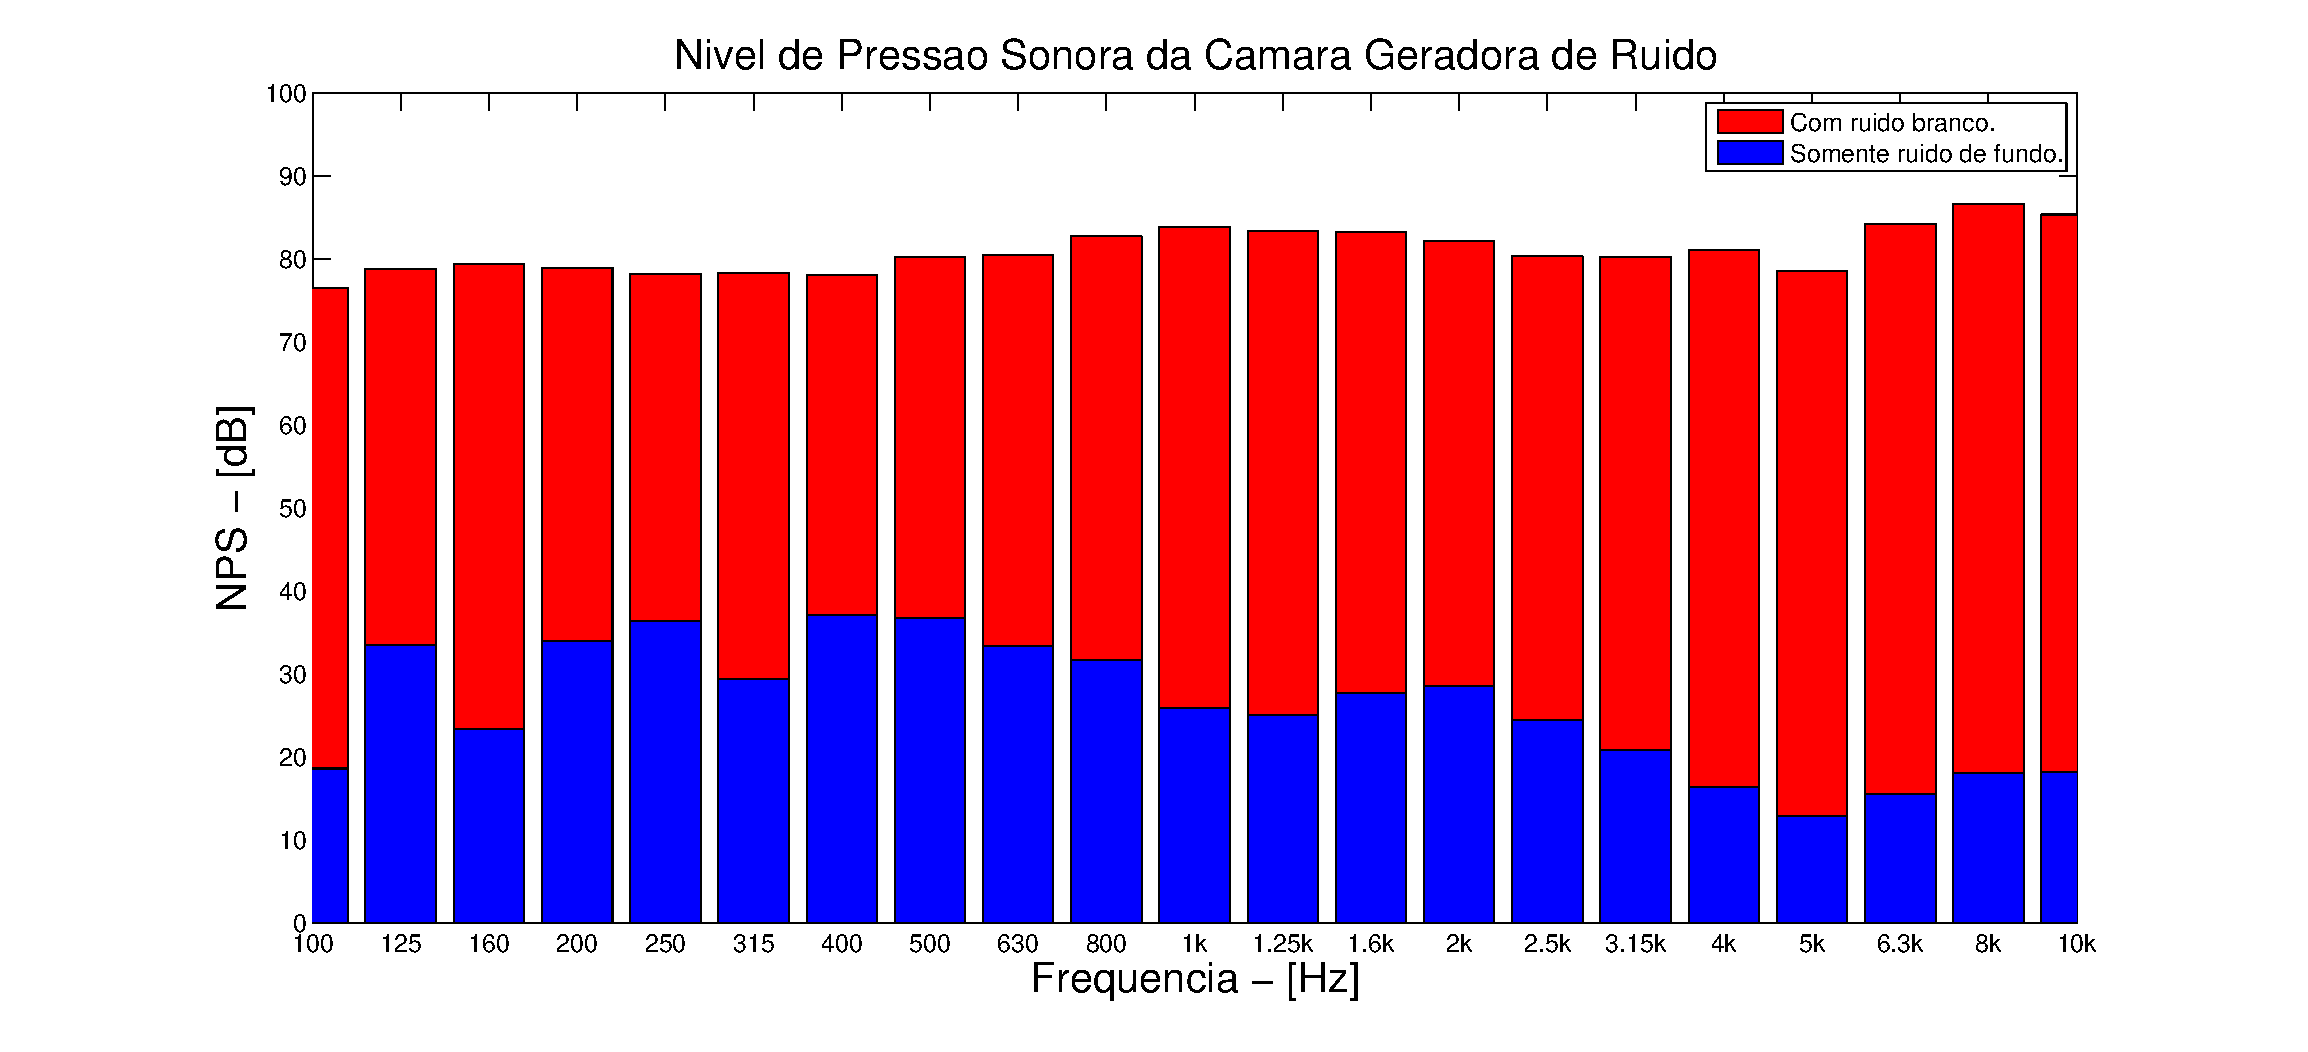
\includegraphics[width=40cm,height=40cm,keepaspectratio]{codigo/pressao_sonora_geradora.eps}
	\caption{Esquemático do acoplamento das camaras I e II. Fonte: \cite{silva2009simulaccao}}
	\label{experimento_1}
\end{figure}

\newpage
Segue as dimensões das câmaras I e II na figura \ref{experimento_2}.

\begin{figure}[h]
	\centering
	%\hspace{-4.5cm}
	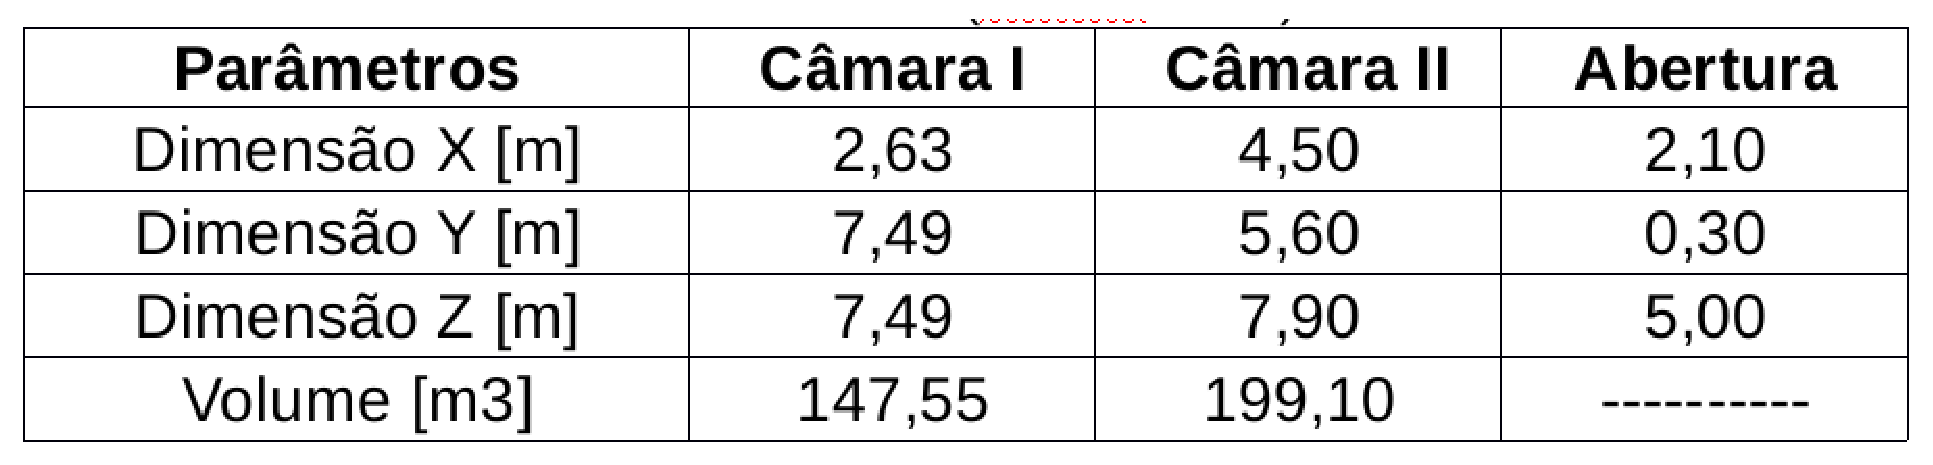
\includegraphics[scale=0.35]{imagem_4.eps}
	%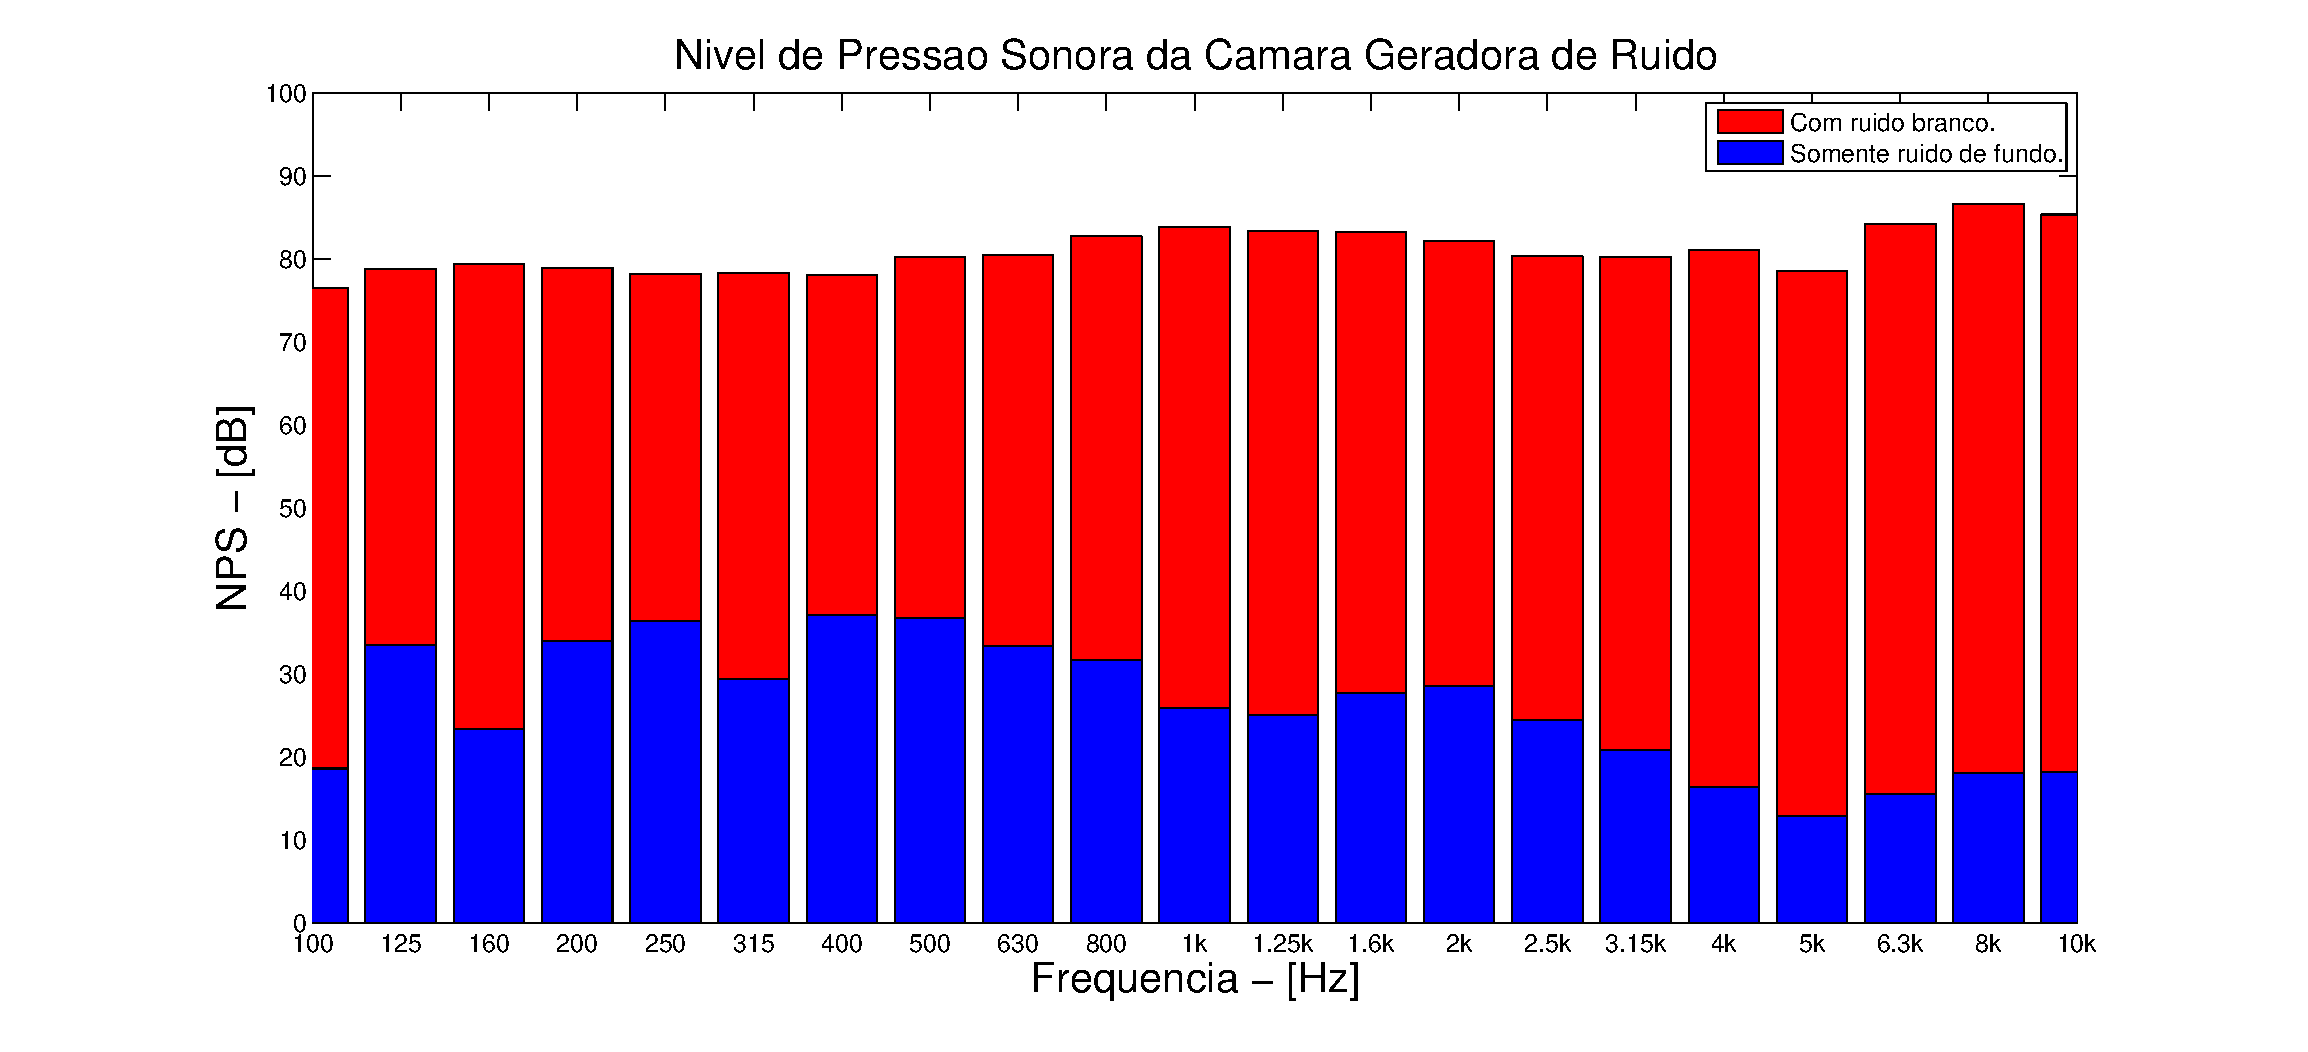
\includegraphics[width=40cm,height=40cm,keepaspectratio]{codigo/pressao_sonora_geradora.eps}
	\caption{Dimensões das câmaras I e II. Fonte: \cite{silva2009simulaccao}}
	\label{experimento_2}
\end{figure}

Segue os tempos de reverberação das câmaras I e II na figura \ref{experimento_3}.
\begin{figure}[h]
	\centering
	%\hspace{-4.5cm}
	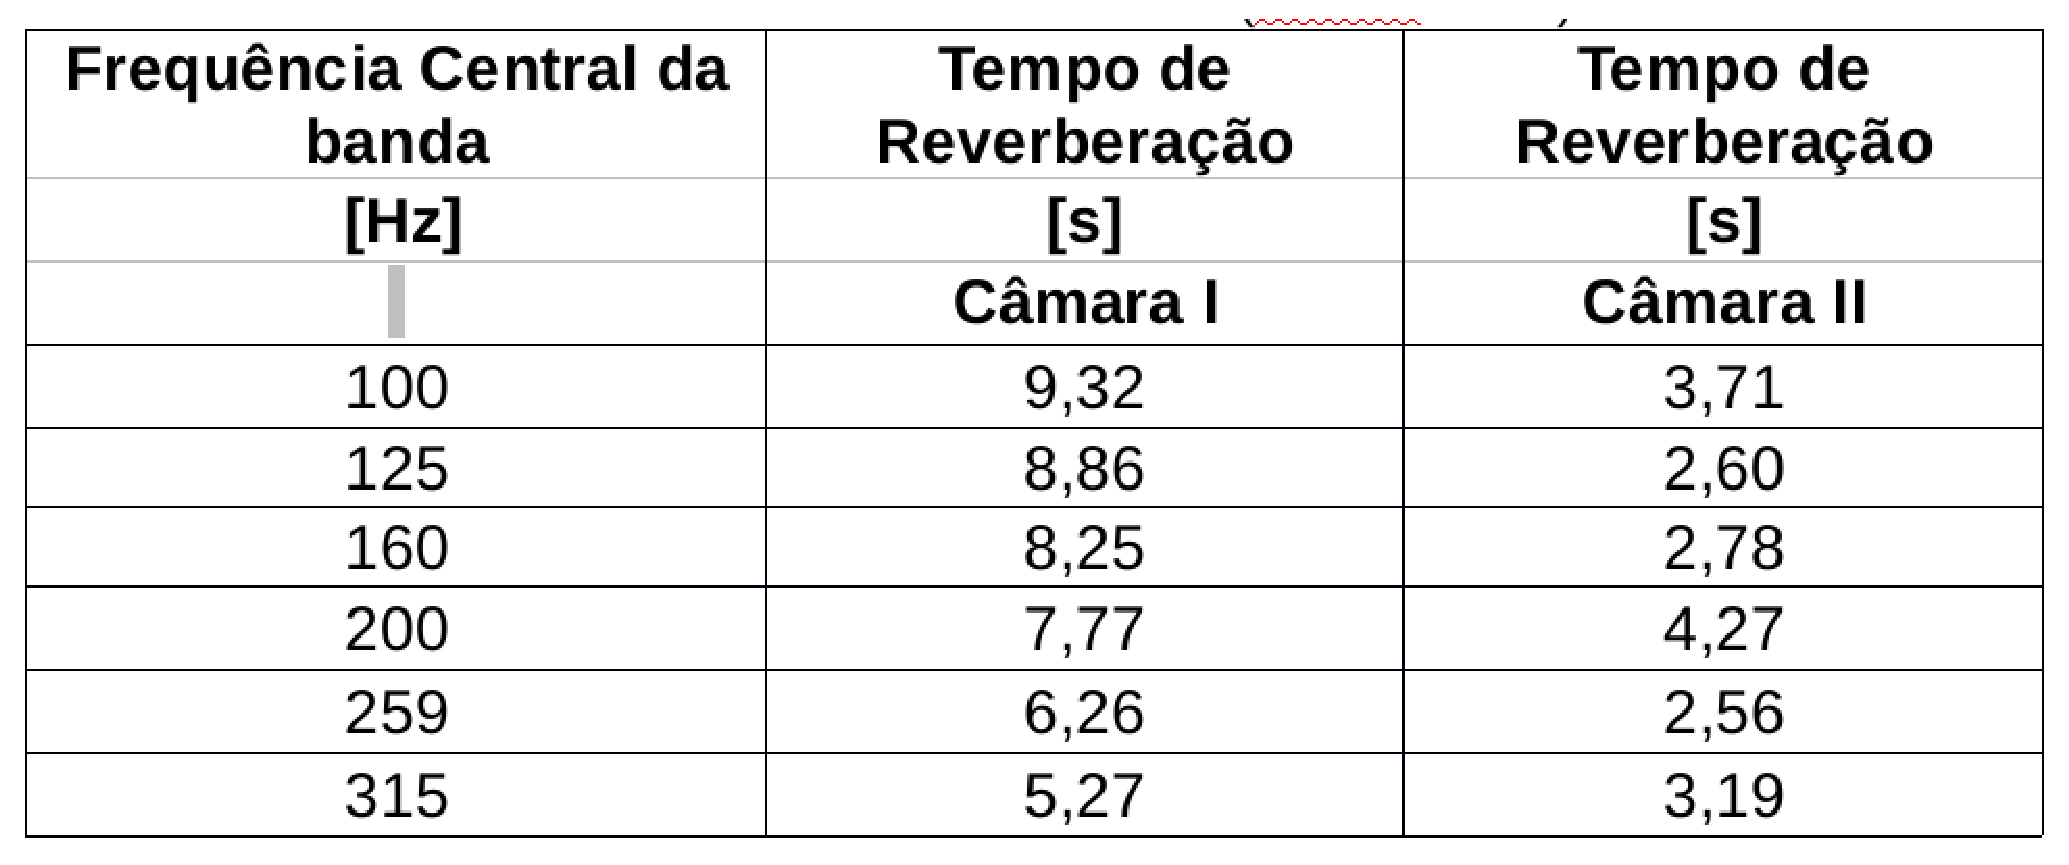
\includegraphics[scale=0.35]{imagem_5.eps}
	%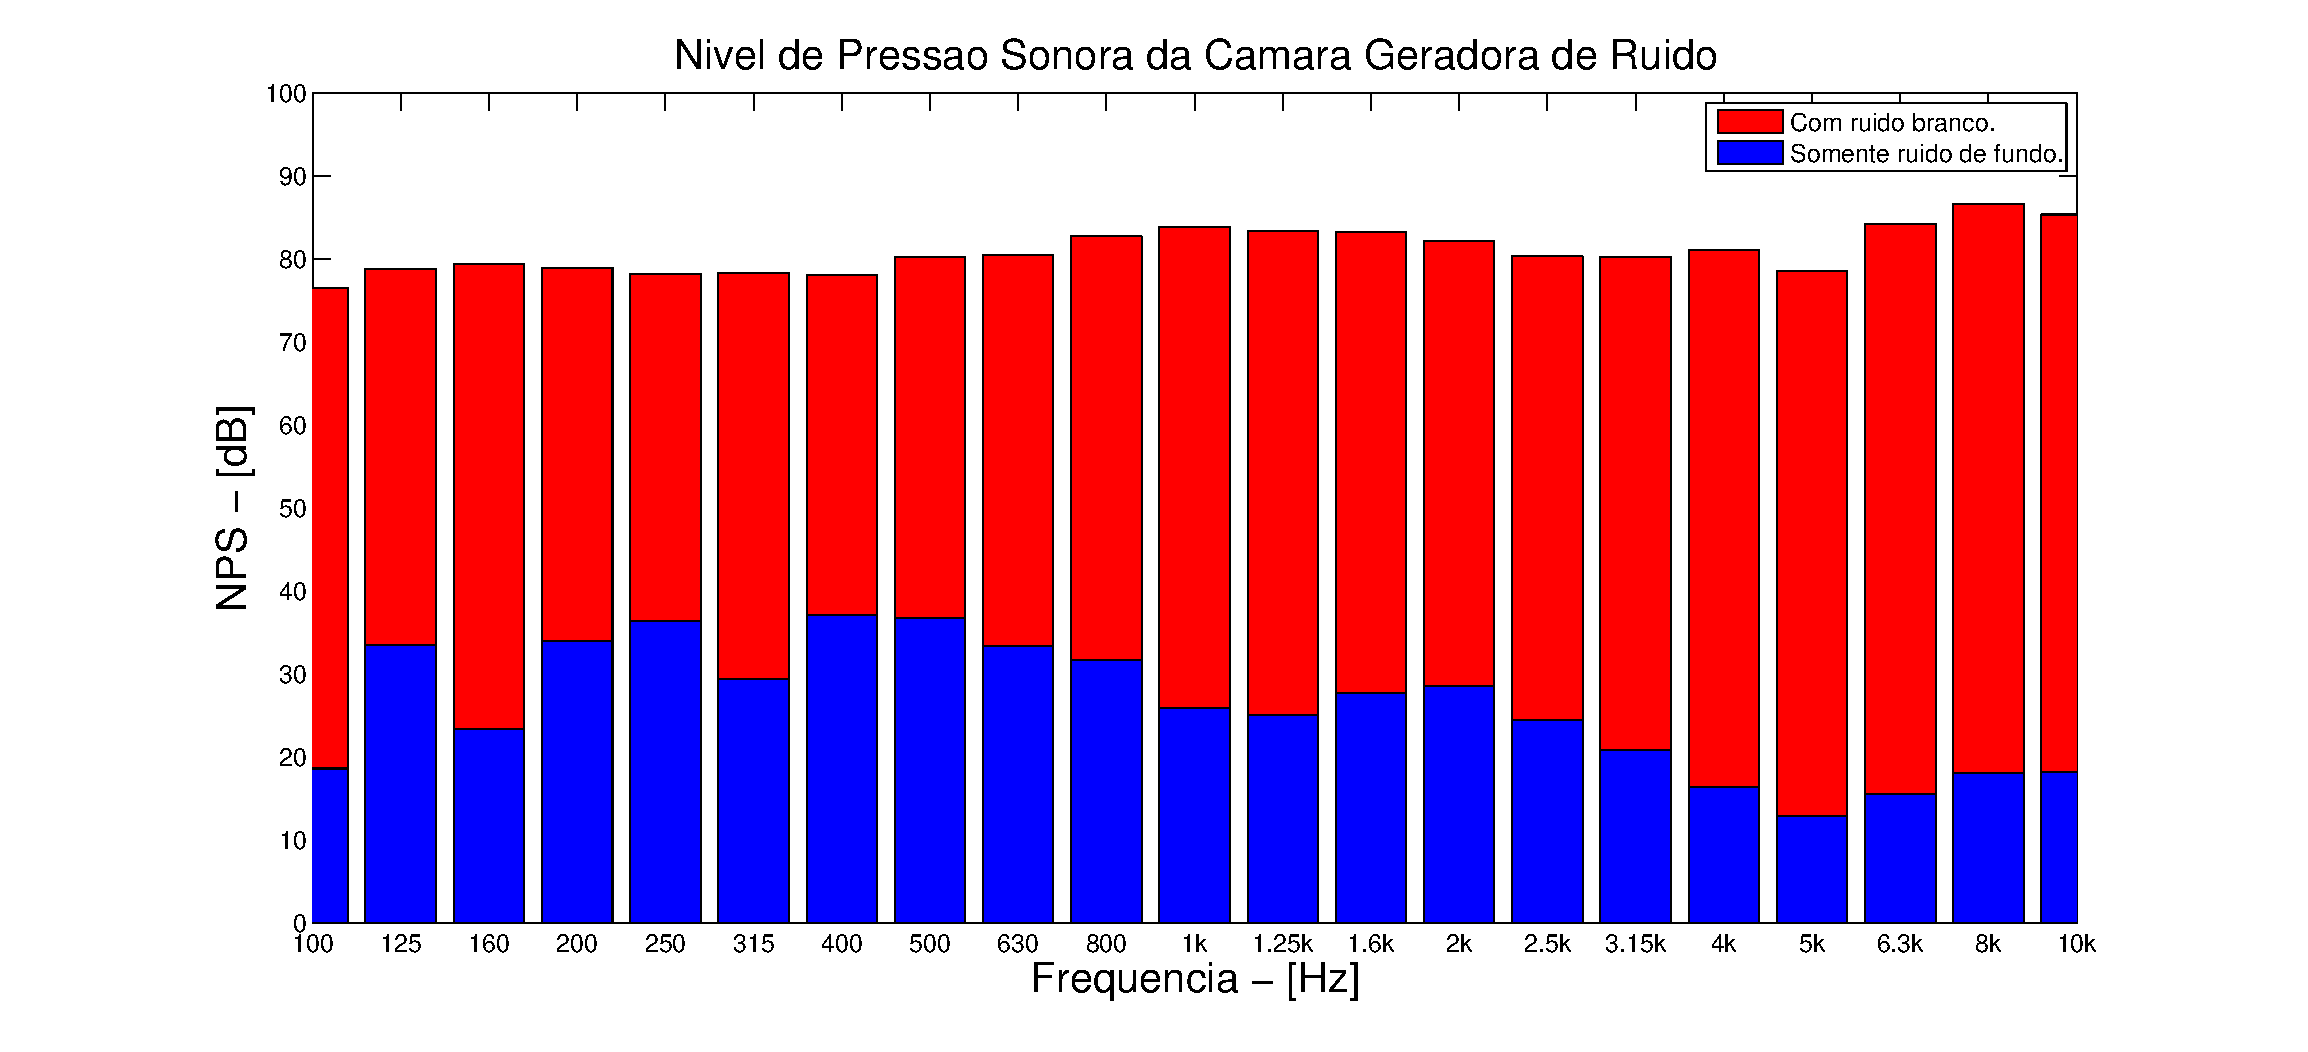
\includegraphics[width=40cm,height=40cm,keepaspectratio]{codigo/pressao_sonora_geradora.eps}
	\caption{Tempos de reverberação das câmaras I e II. Fonte: \cite{silva2009simulaccao}}
	\label{experimento_3}
\end{figure}

\newpage
Segue disposição experimental da câmara I geradora na figura \ref{experimento_4}.
\begin{figure}[h]
	\centering
	%\hspace{-4.5cm}
	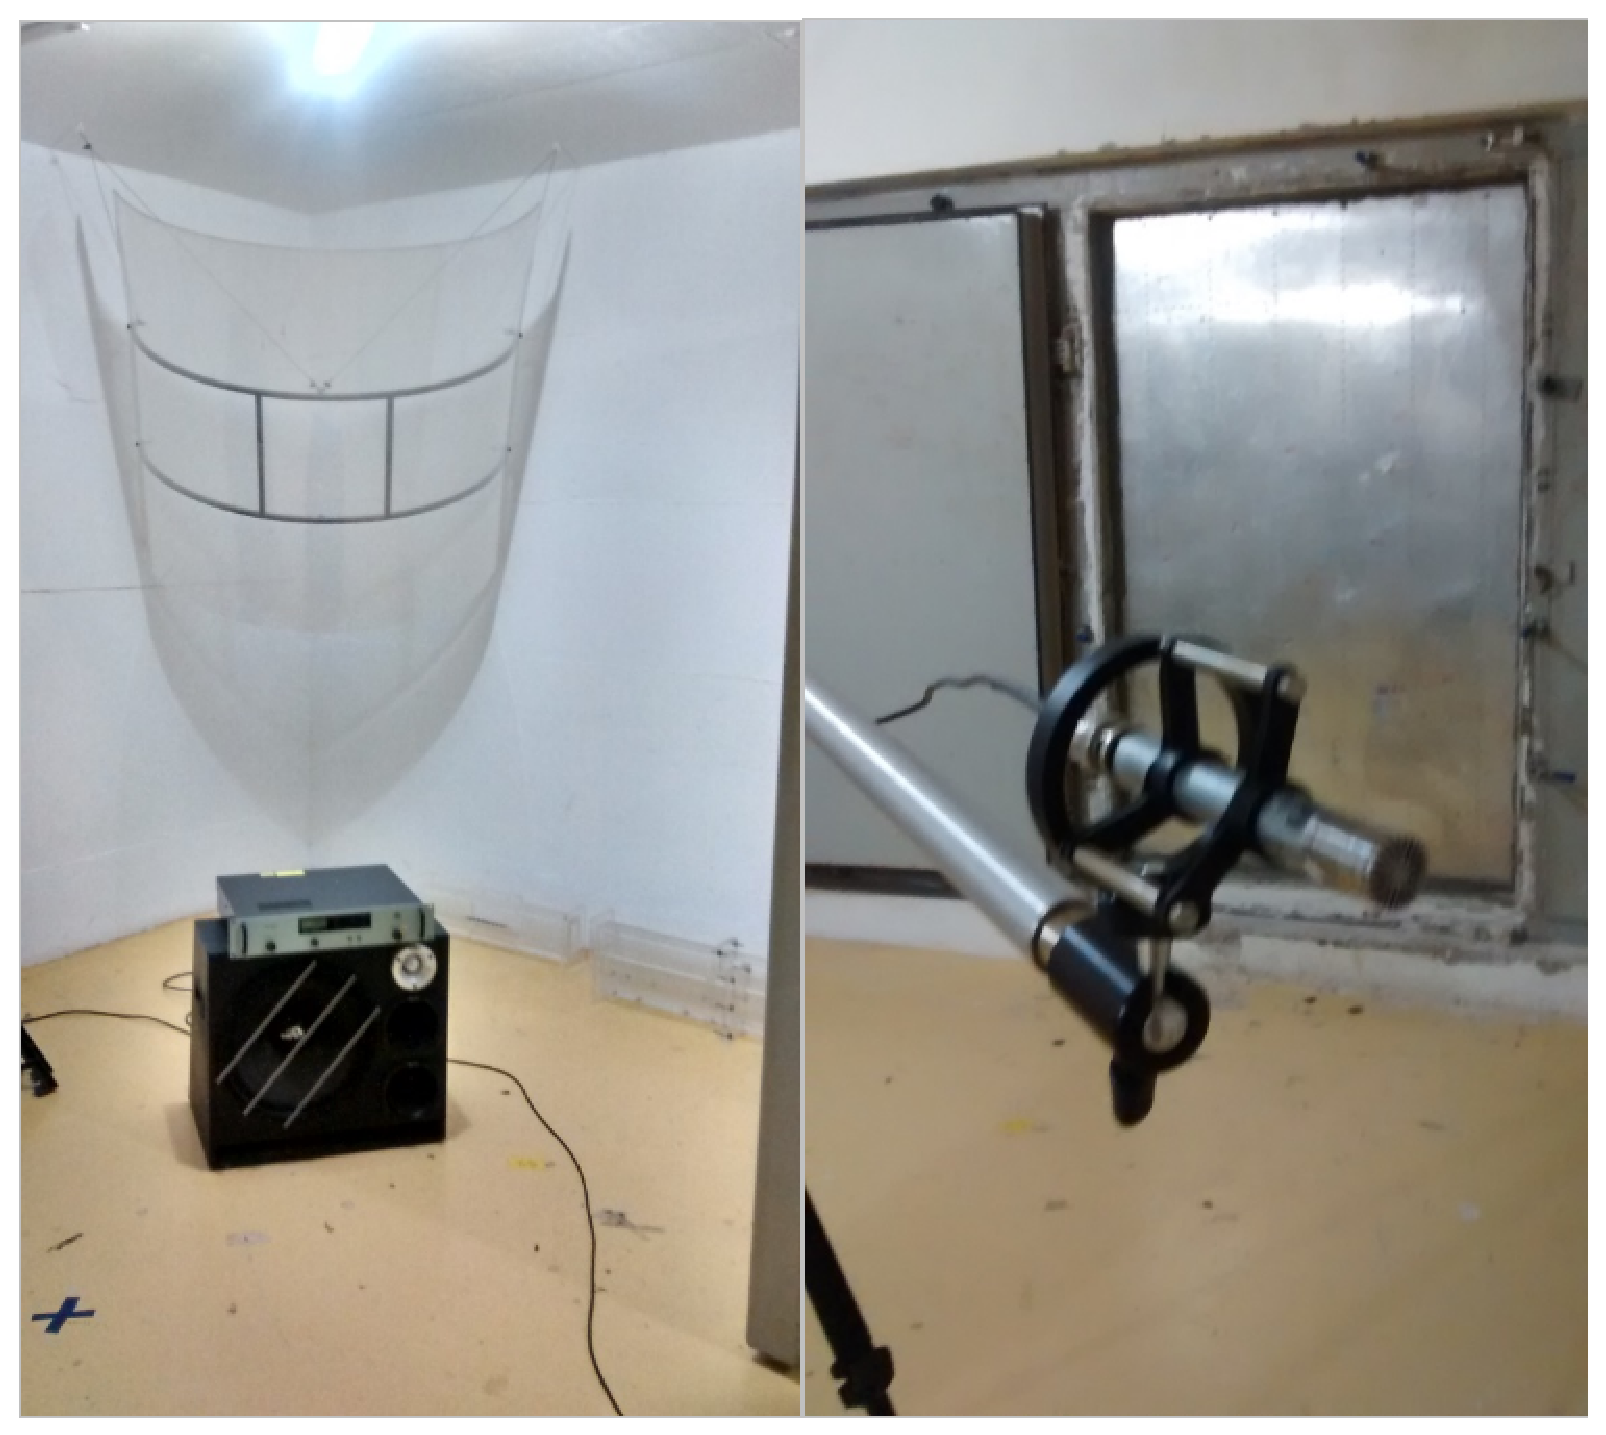
\includegraphics[scale=0.35]{imagem_2.eps}
	%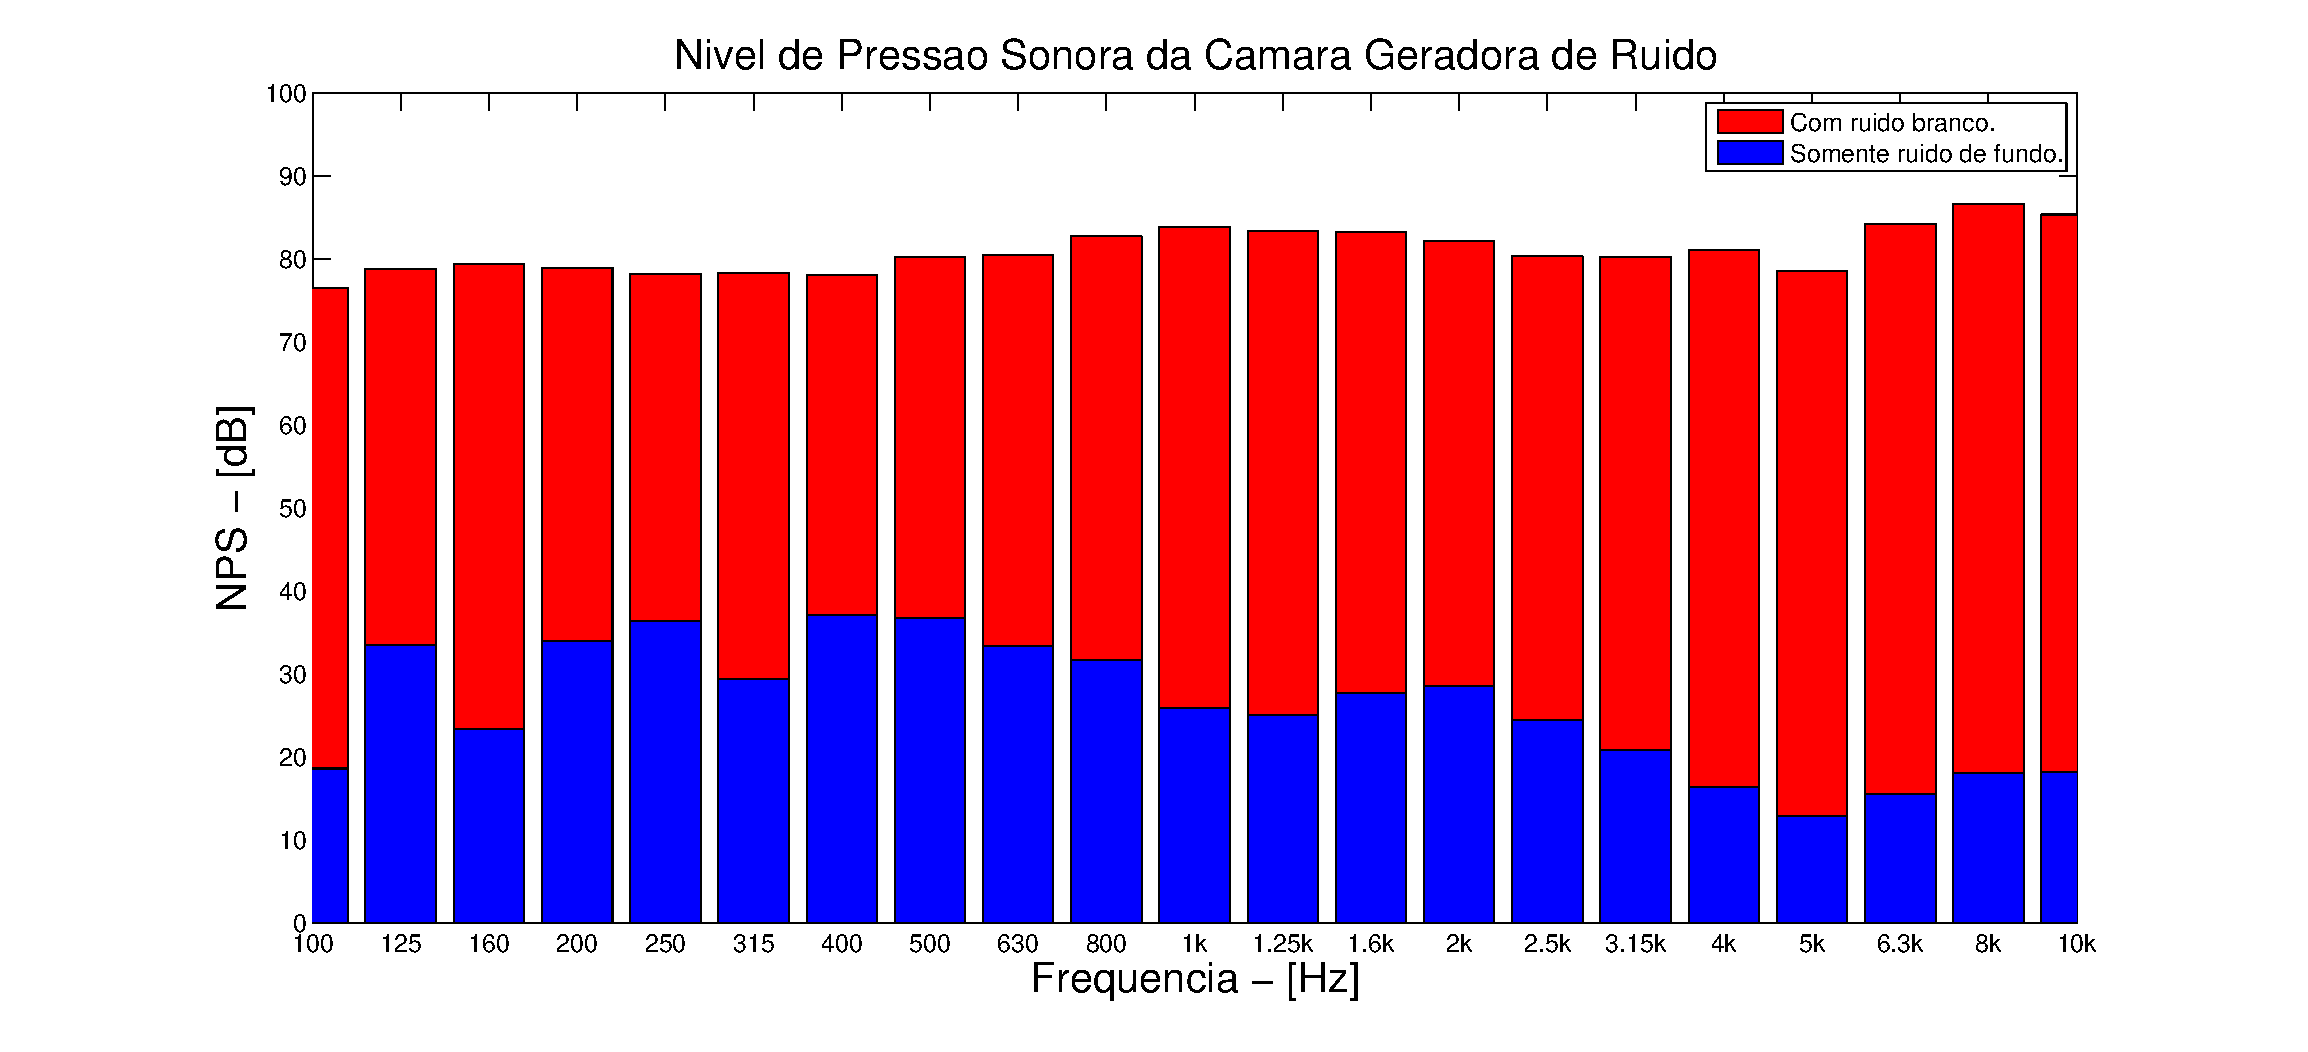
\includegraphics[width=40cm,height=40cm,keepaspectratio]{codigo/pressao_sonora_geradora.eps}
	\caption{Câmara I. Fonte: \cite{silva2009simulaccao}}
	\label{experimento_4}
\end{figure}

Segue disposição experimental da câmara I geradora na figura \ref{experimento_5}.
\begin{figure}[h]
	\centering
	%\hspace{-4.5cm}
	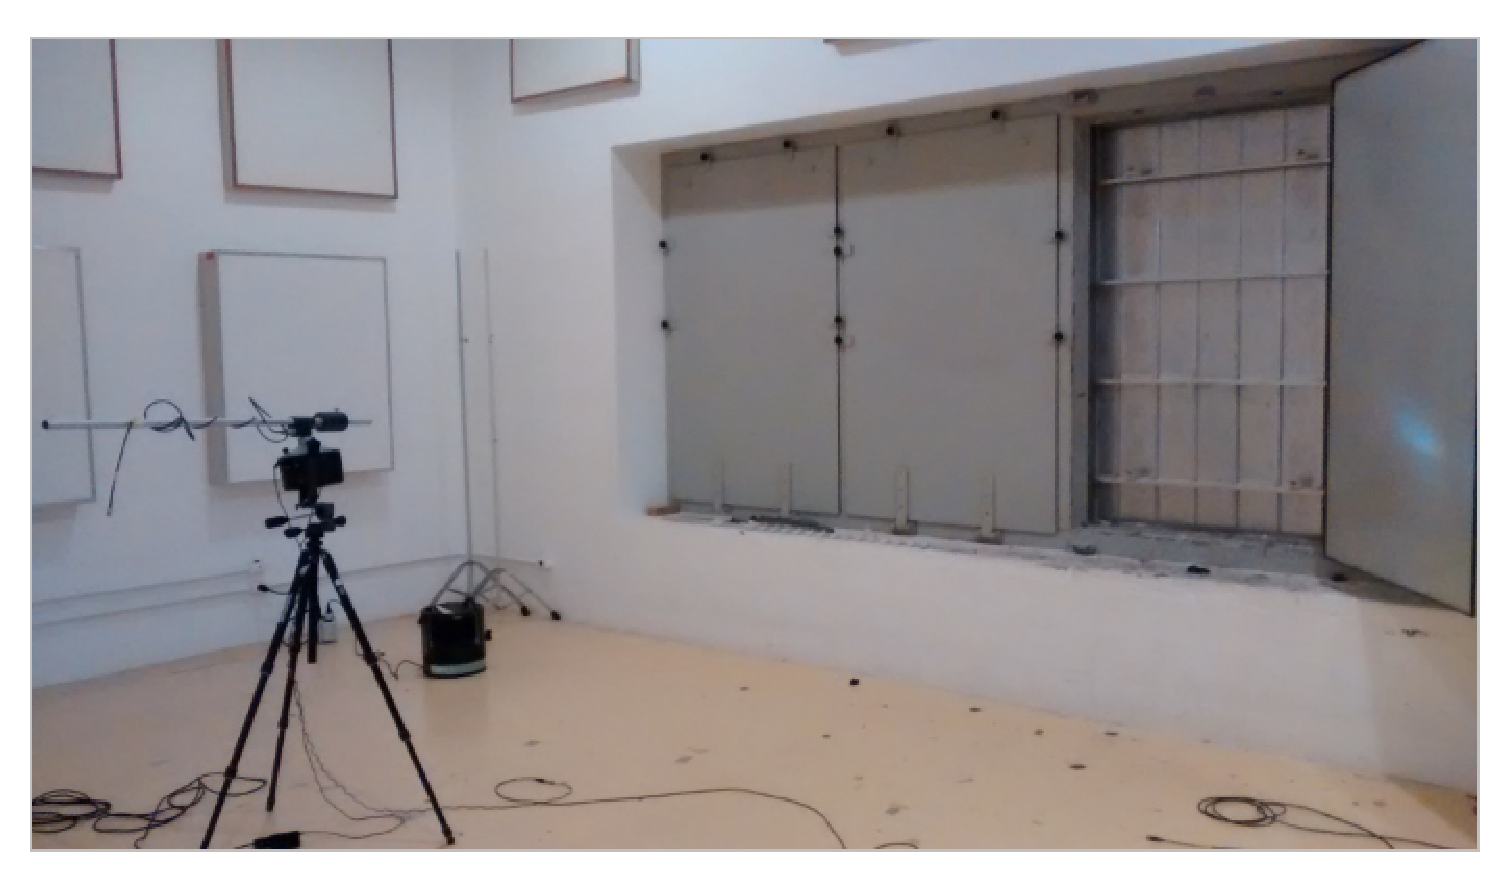
\includegraphics[scale=0.35]{imagem_1.eps}
	%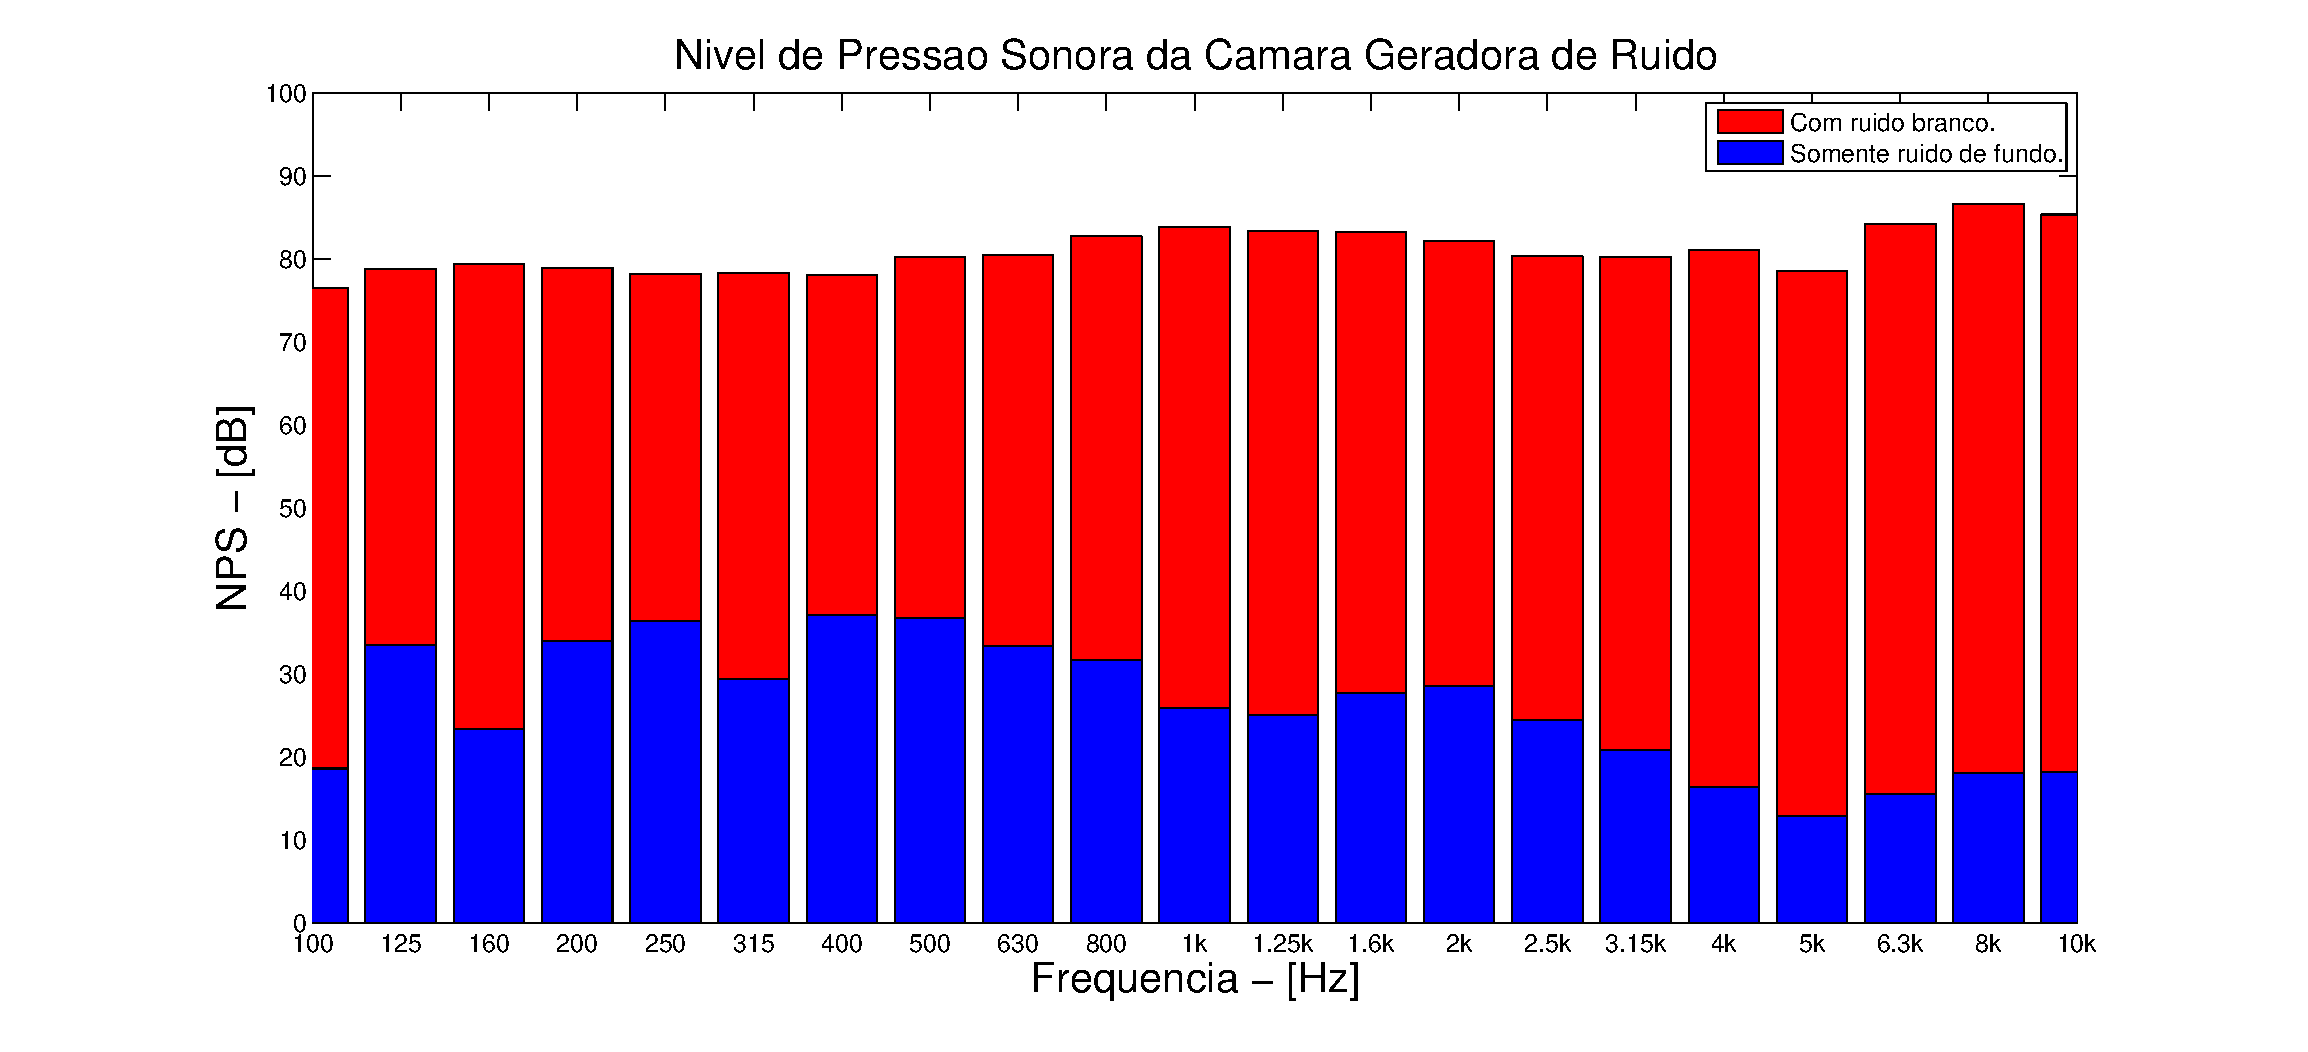
\includegraphics[width=40cm,height=40cm,keepaspectratio]{codigo/pressao_sonora_geradora.eps}
	\caption{Câmara II. Fonte: \cite{silva2009simulaccao}}
	\label{experimento_5}
\end{figure}

\chapter{Resultados}\label{resultados}

No que diz respeteito aos resultados do experimento abordado, foram consolidados o espectro de frequências do ruído branco e do ruído de fundo nas salas geradoras e receptoras respectivamente e, como resultado principal, foi extraído a perda de transmissão em relação as frequências por 2 métodos, o indireto (por comparação) e direto (por sabine, usando o tempo de reverberação da câmara).

\begin{figure}[h]
%\centering
\hspace{-4.5cm}
%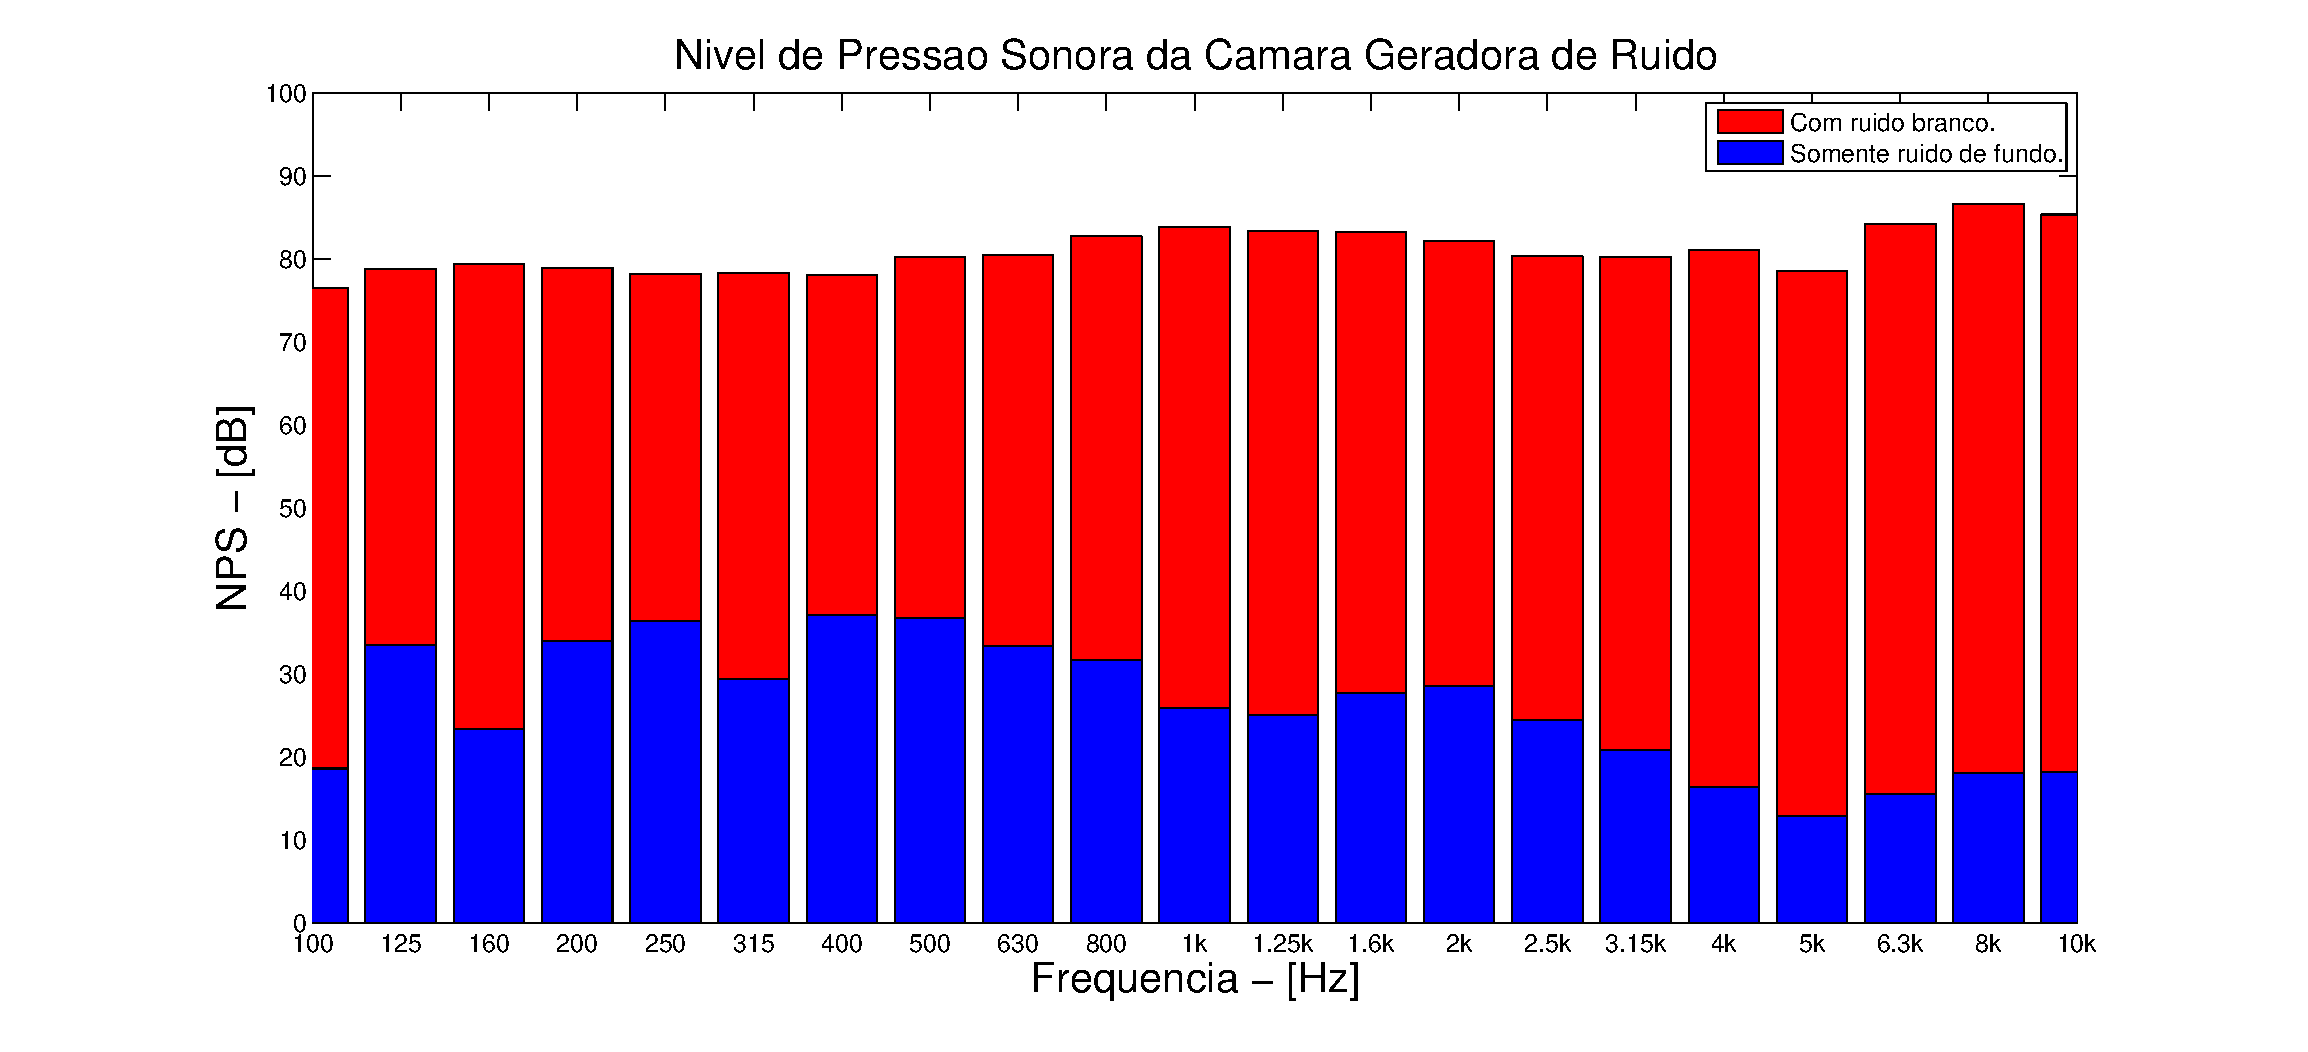
\includegraphics[scale=0.6]{codigo/pressao_sonora_geradora.eps}
%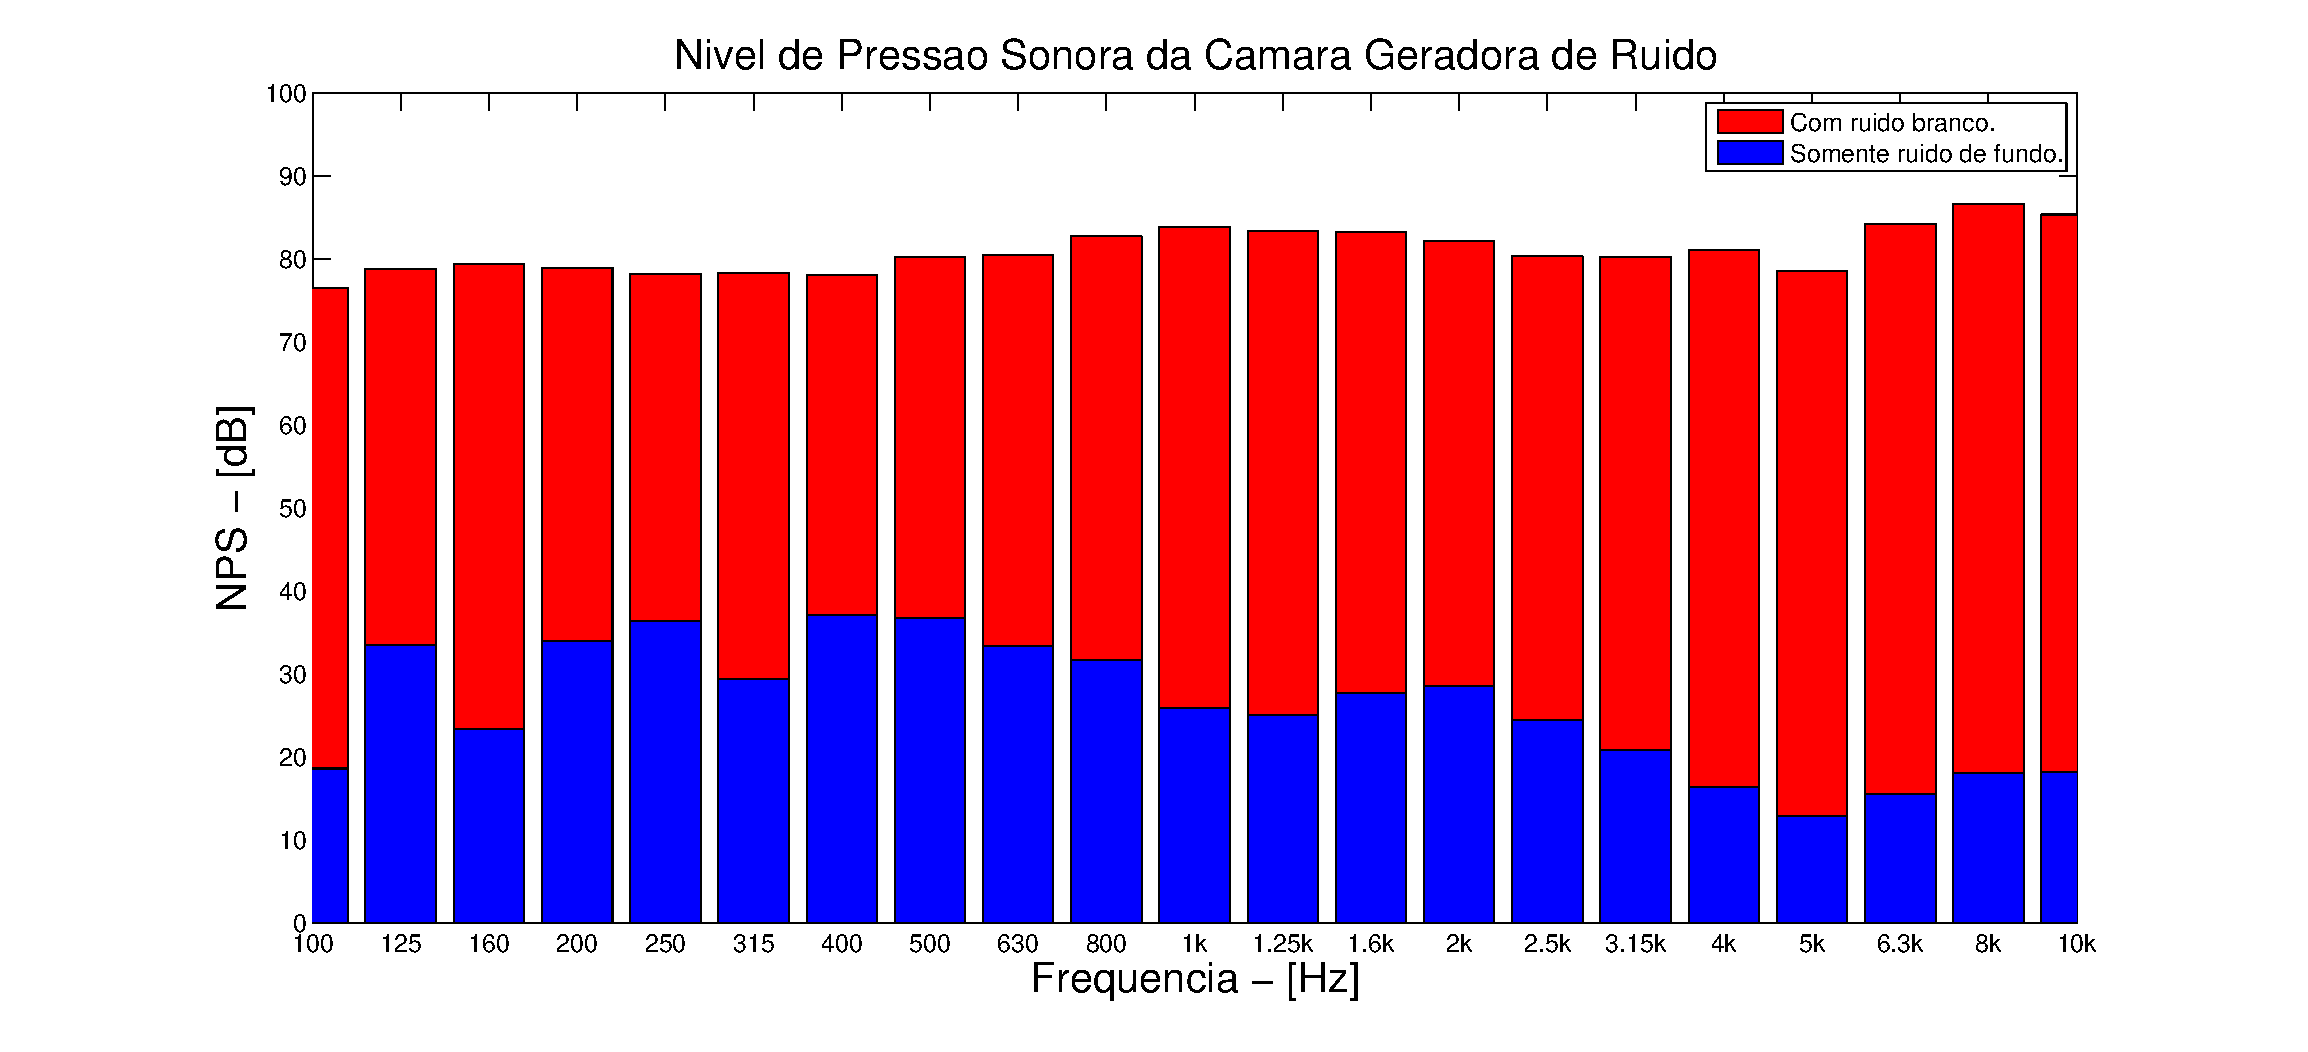
\includegraphics[width=40cm,height=40cm,keepaspectratio]{codigo/pressao_sonora_geradora.eps}
\caption{Níveis de pressão sonora na câmara geradora de ruído branco.}
\label{resultado_1}
\end{figure}

Diante do que é exposto no gráfico da figura \ref{resultado_1} é perceptível que o ruído branco se sobressaiu mais que 15 dB em relação ao ruído de fundo. Esse fato corrobora com uma medida sem necessidades de correção, pelo que é exposto em \cite{silva2009simulaccao}.

\newpage
\begin{figure}[h]
%\centering
\hspace{-4.5cm}
%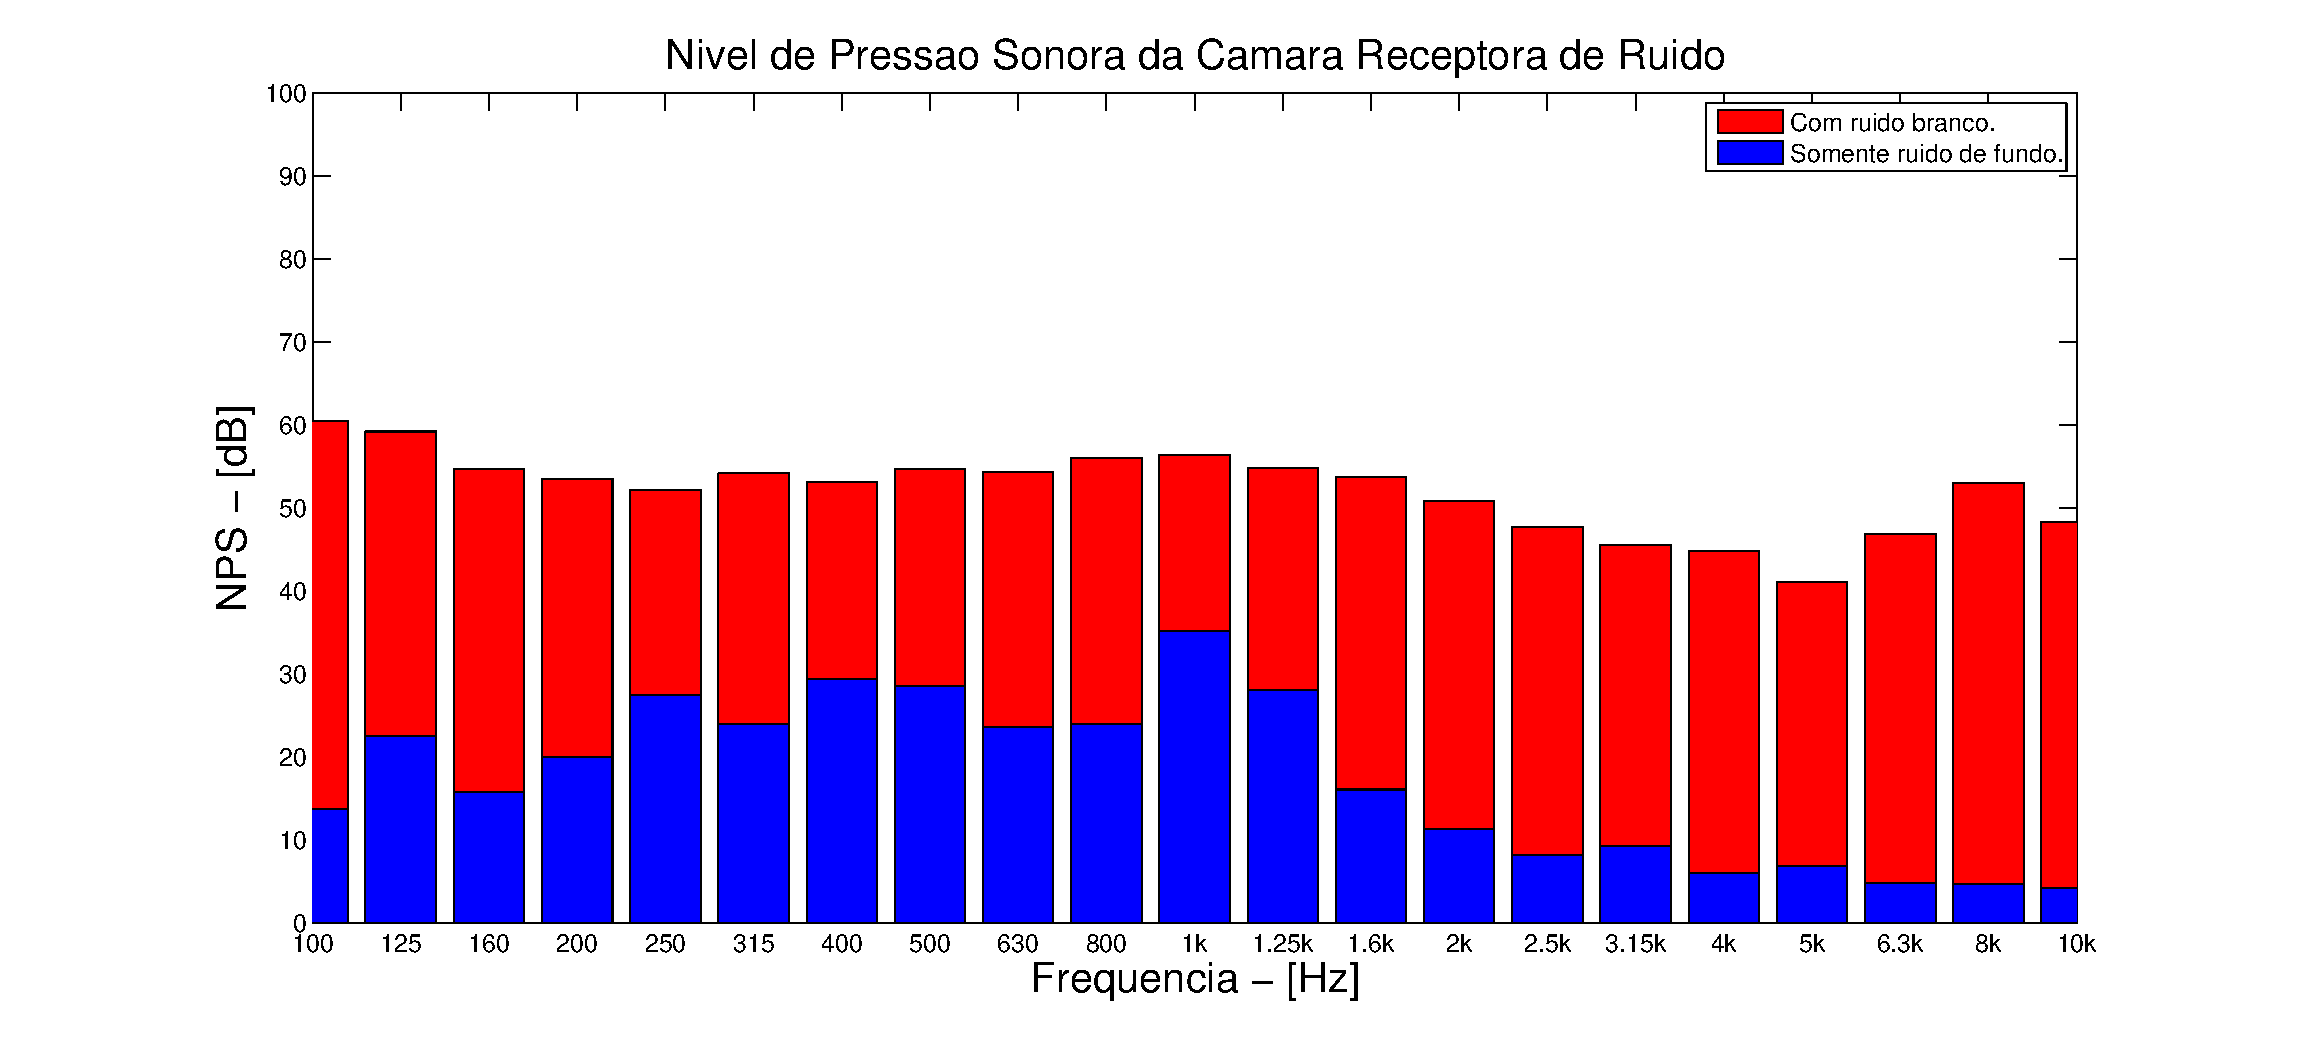
\includegraphics[scale=0.6]{codigo/pressao_sonora_receptora.eps}
\caption{Níveis de pressão sonora na câmara receptora de ruído branco.}
\label{resultado_2}
\end{figure}

Diante do que é exposto no gráfico da figura \ref{resultado_2} é perceptível que o ruído branco se sobressaiu mais que 15 dB em relação ao ruído de fundo. Esse fato corrobora com uma medida sem necessidades de correção, pelo que é exposto em \cite{silva2009simulaccao}.

\newpage
\begin{figure}[h]
%\centering
\hspace{-4.5cm}
%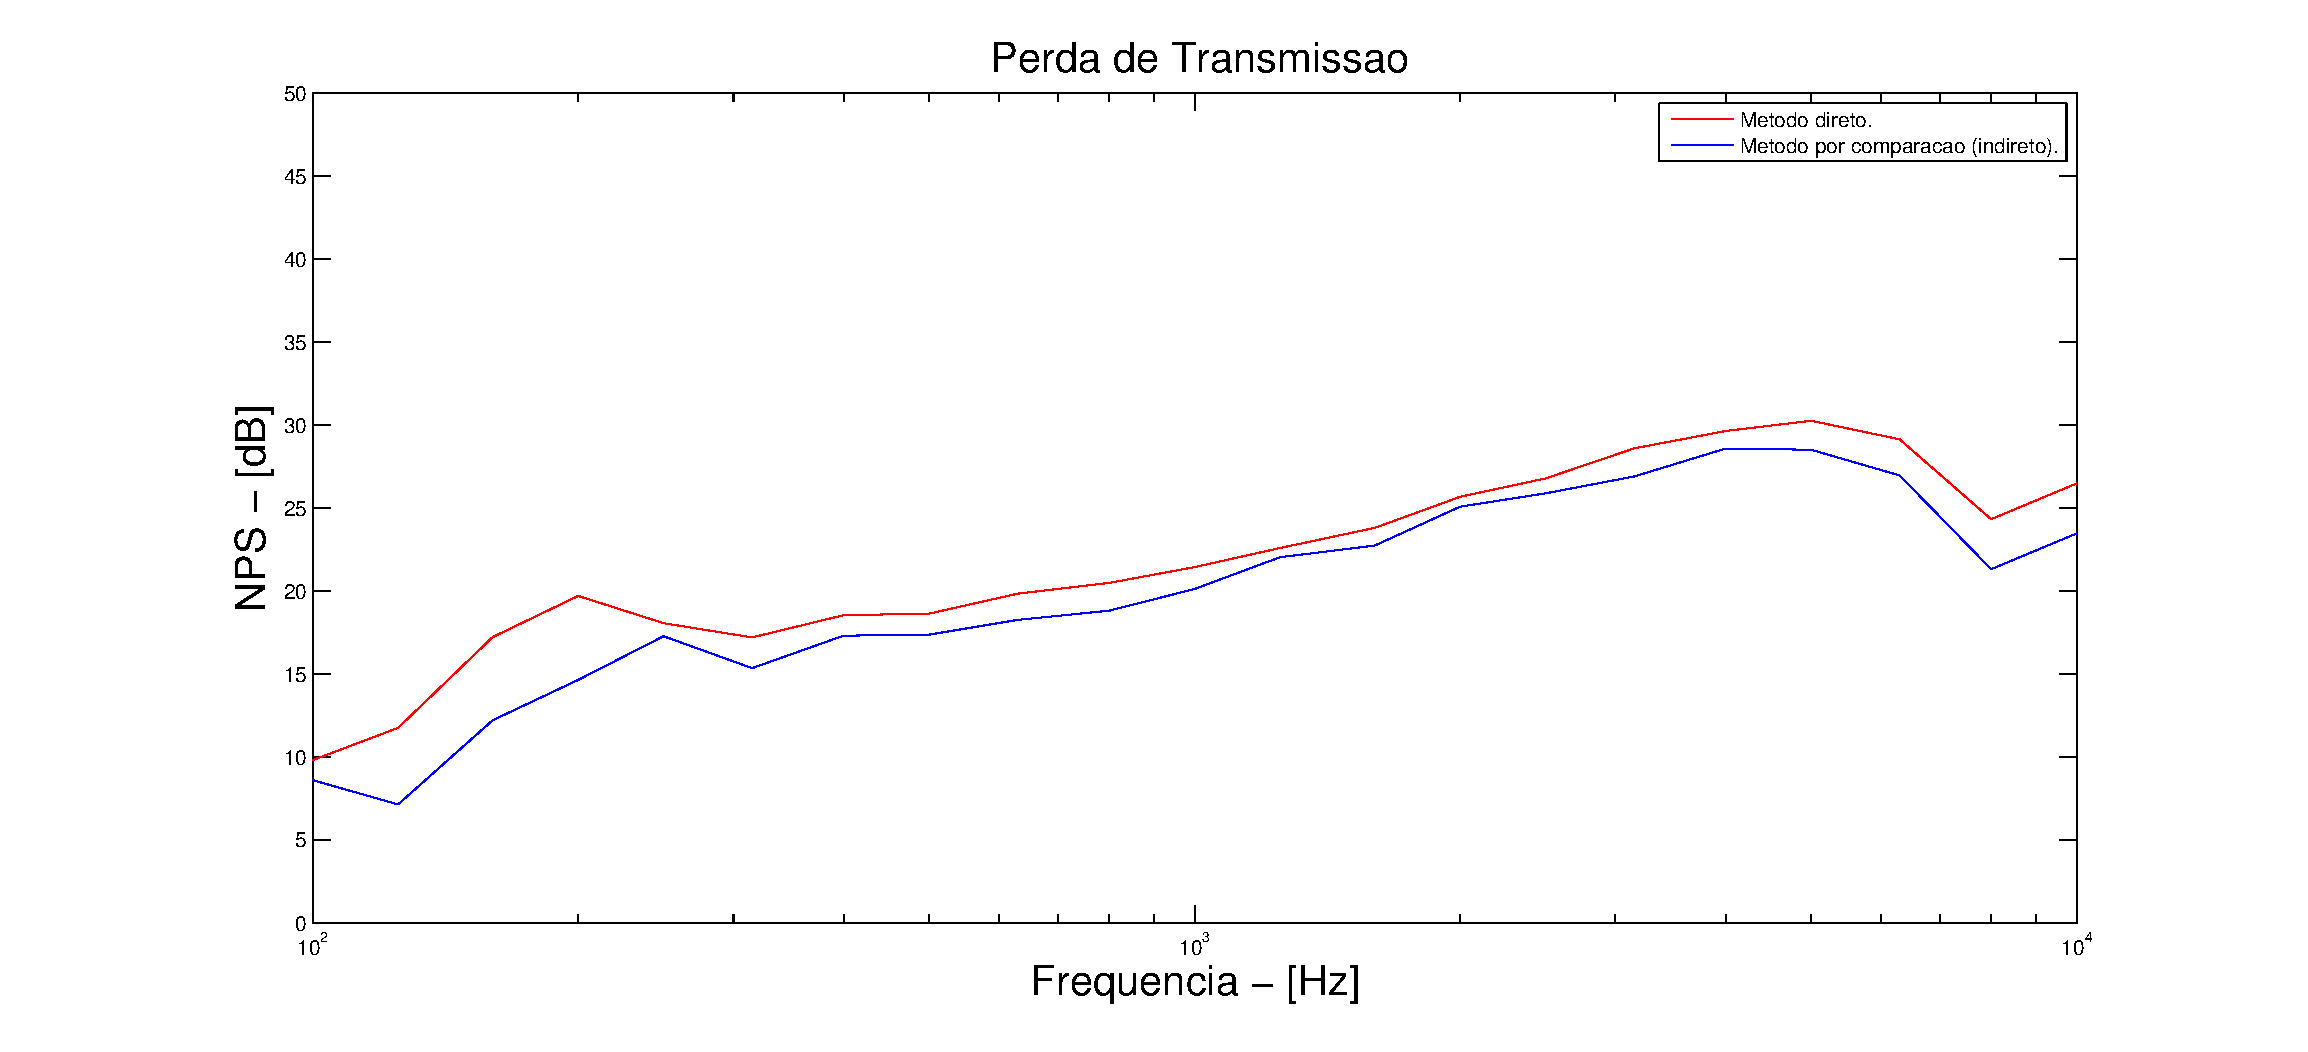
\includegraphics[scale=0.6]{codigo/perda_transmissao.eps}
\caption{Gráfico de perda de transmissão da placa de alumínio.}
\label{resultado_3}
\end{figure}

A figura \ref{resultado_3} mostra o resultado principal do experimento: a perda de transmissão em relação a frequência. É perceptível que, a medida que a placa é exposta para altas frequências, há uma perda maior. E esse fato corrobora com o que é medido pelo método indireto (feito por tempo de reverberação). As extremidades do gráfico, onde aparecem as curvas, dizem respeito ao regime elástico de comportamento, a parte linear diz respeito ao regime rígido da placa.


\chapter{Conclusões}\label{conclusoes}

O experimento descrito anteriormente reforçou as particularidades do uso de uma placa de alumínio naval para perda de transmissão. Observa-se que a medida que a frequência aumenta, maior é a perda de transmissão para ambos os métodos de cálculo de área de absorção: direto e indireto. Os resultados poderiam ser mais acurados com uma placa totalmente lisa.